%!TEX root = ../dissertation.tex

\hypertarget{(chap:capitolo4)}{}
\chapter{Moduli Food-and-beverage}
In questo capitolo presenteremo prima una rapida introduzione ai moduli odoo, tratta dalla
\bit{documentazione}{doc} degli sviluppatori, per poi analizzare nel dettaglio ciascun modulo implementato, spiegando ciascun vincolo e delineandone quindi l'idea di base.
\section{Modulo odoo standard}
Odoo usa un'architettura client/server nella quale i client sono web browser che accedo al server odoo tramite \glo{RPC}.
La logica aziendale e l'estensione vengono generalmente eseguite sul lato server.
Entrambe le estensioni server e client sono impacchettate come moduli che possono essere caricati facoltativamente in un database. I moduli Odoo possono sia aggiungere una nuovissima logica aziendale a un sistema Odoo, sia alterare ed estendere la logica aziendale esistente.\\
Tutto in Odoo quindi inizia e termina con i moduli.


\subsection{Composizione di un modulo}
Un modulo Odoo può contenere un numero di elementi:
\newpage
\begin{itemize}
	\item \textbf{Oggetti business} Dichiarate come classi Python, queste risorse vengono automaticamente mantenute da Odoo in base alla loro configurazione
	\item \textbf{File di dati} File XML o CSV che dichiarano metadati (viste o report), dati di configurazione (parametrizzazione dei moduli), dati dimostrativi e altro
	\item \textbf{Controller Web} Gestire le richieste dai browser Web
	\item \textbf{Dati web statici} Immagini, file CSS o javascript utilizzati dall'interfaccia Web o dal sito Web
\end{itemize}

\subsection{Struttura di un modulo}
Ogni modulo è una directory all'interno di una directory contenente tutti i moduli Odoo, specificata utilizzando il comando "- -addons-path <nome\_modulo>" nel file di configurazione.
\begin{figure}[H]
	\begin{center} 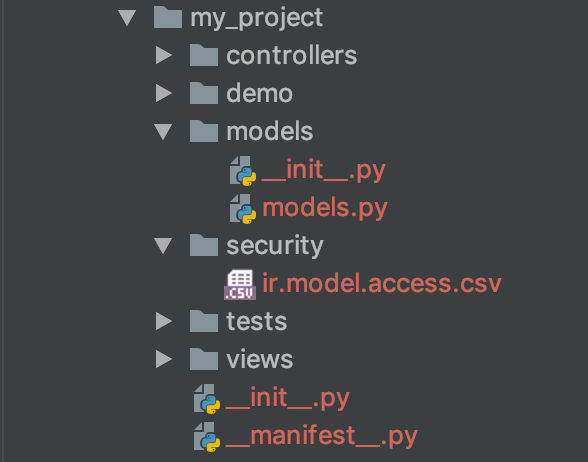
\includegraphics[scale=0.5]{figures/structure_odoo}
		\caption[Struttura di un modulo]{Struttura modulo}
		\label{fig:structure_odoo}
	\end{center}
\end{figure}

Un modulo è dichiarato nel suo file "\_manifest\_.py", per specificare i metadati del modulo, e anche su un file Python "init.py", contenente l'importazione del controller e modello.
\begin{figure}[H]
	\begin{center} 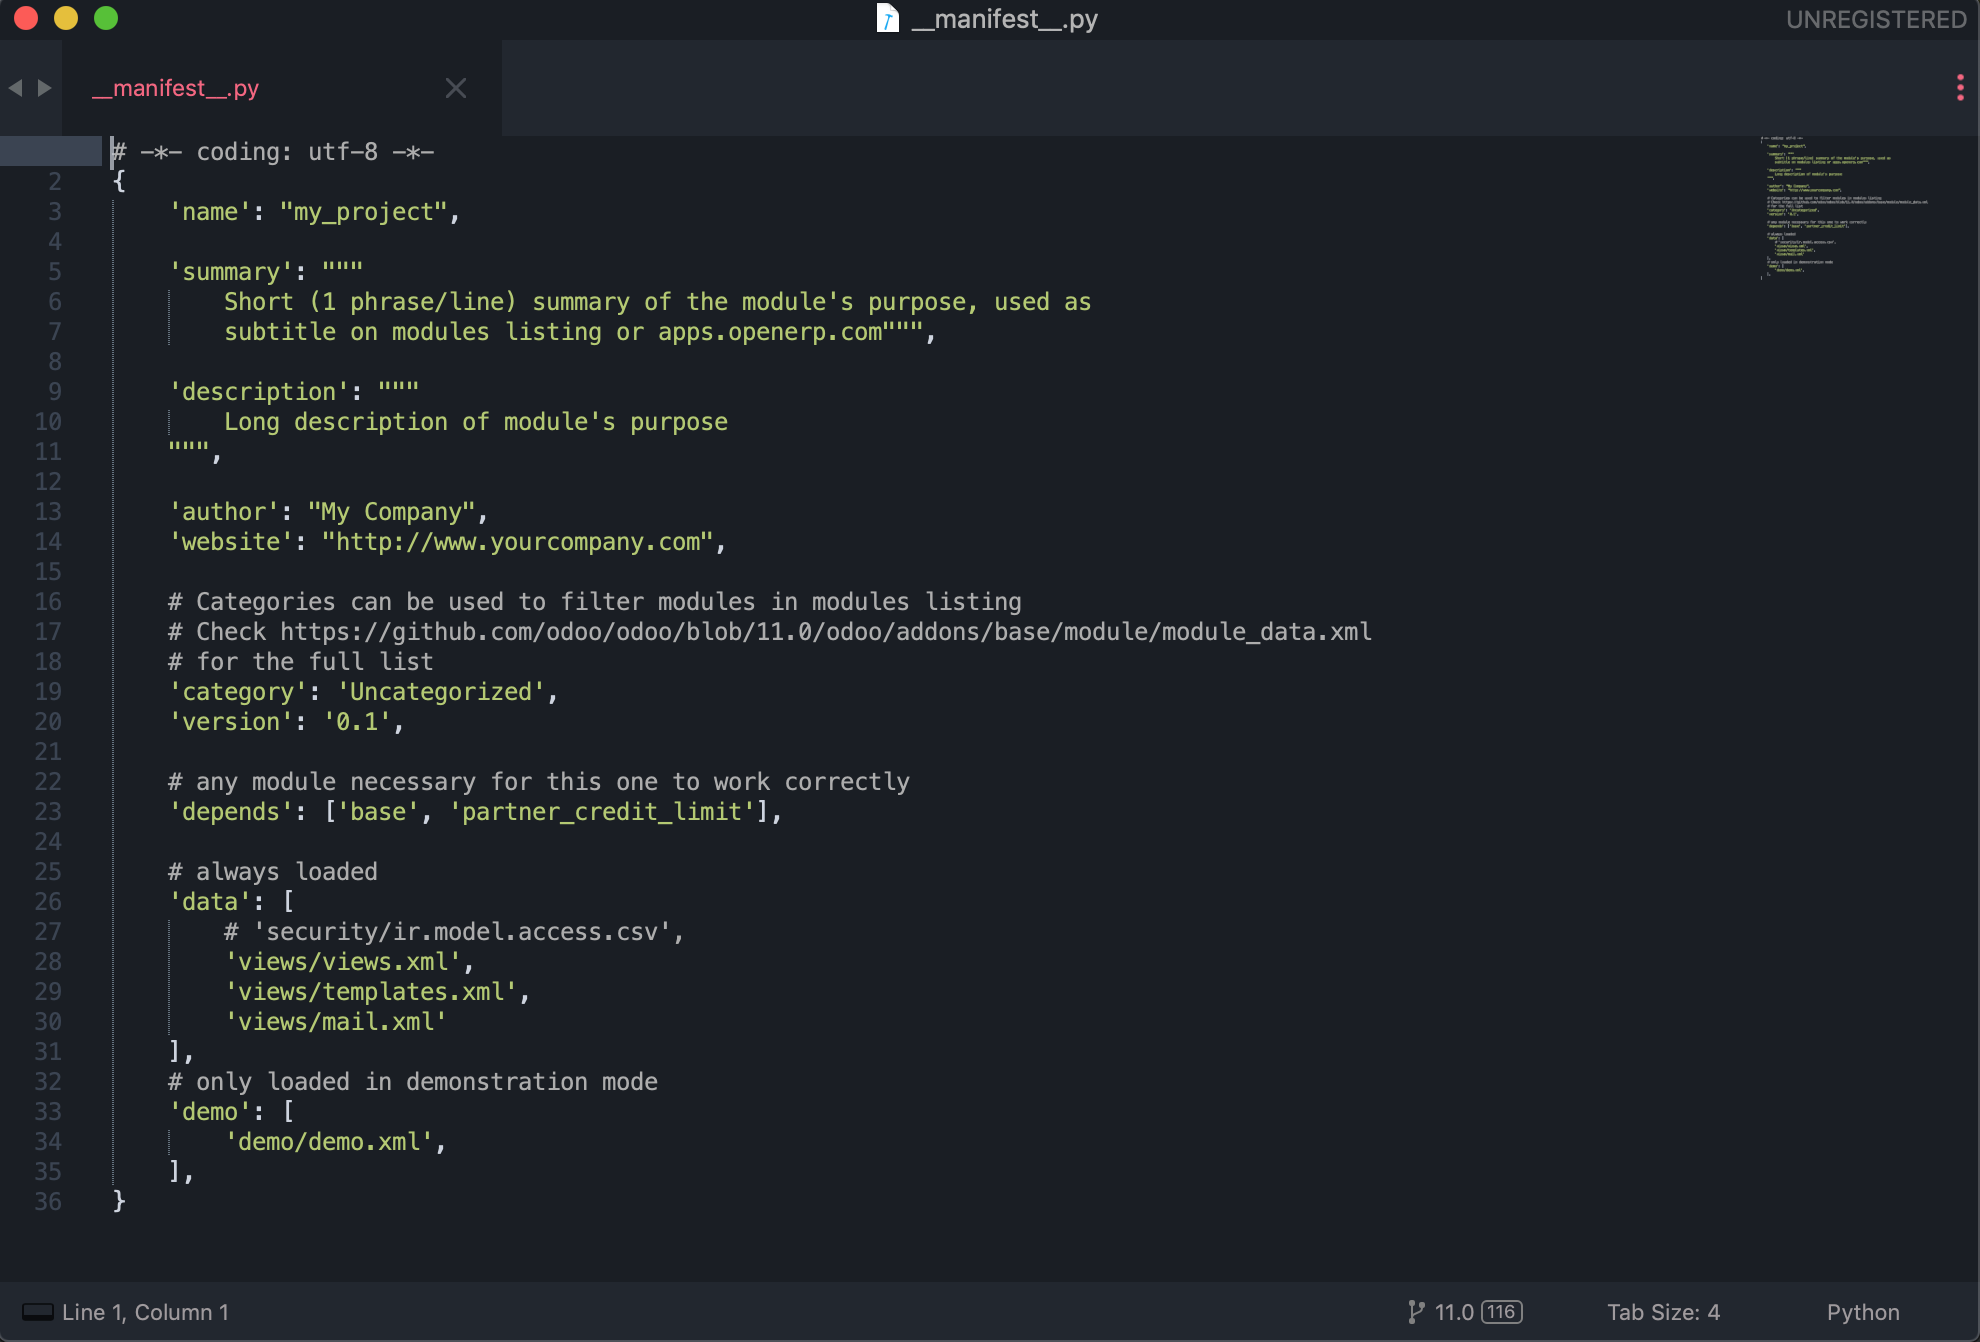
\includegraphics[scale=0.4]{figures/manifest}
		\caption[File manifest]{File manifest}
		\label{fig:manifest}
	\end{center}
\end{figure}

Odoo fornisce un comando per configurare un nuovo modulo (vuoto), creando automaticamente un gruppo di file standard. La maggior parte di essi contiene semplicemente codice commentato o XML:
\begin{figure}[H]
	\begin{center} 
\includegraphics[scale=0.6]{figures/scaffold}
		\caption[Comando per configurare un nuovo modulo]{Comando per configurare un nuovo modulo}
		\label{fig:scaffold}
	\end{center}
\end{figure}
\newpage
Ogni modello odoo è identificato con un id (univoco) ed un nome che può essere individuato nelle impostazioni di odoo. Qui potremo individuare tutte le informazioni riguardo un dato modello, ad esempio: chi eredita, che campi contiene, autorizzazioni di accesso e viste. \\
Tutti questi dati permettono oggettivamente di valutare la corretta implementazione e creazione del modello.

\begin{figure}[H]
	\begin{center} 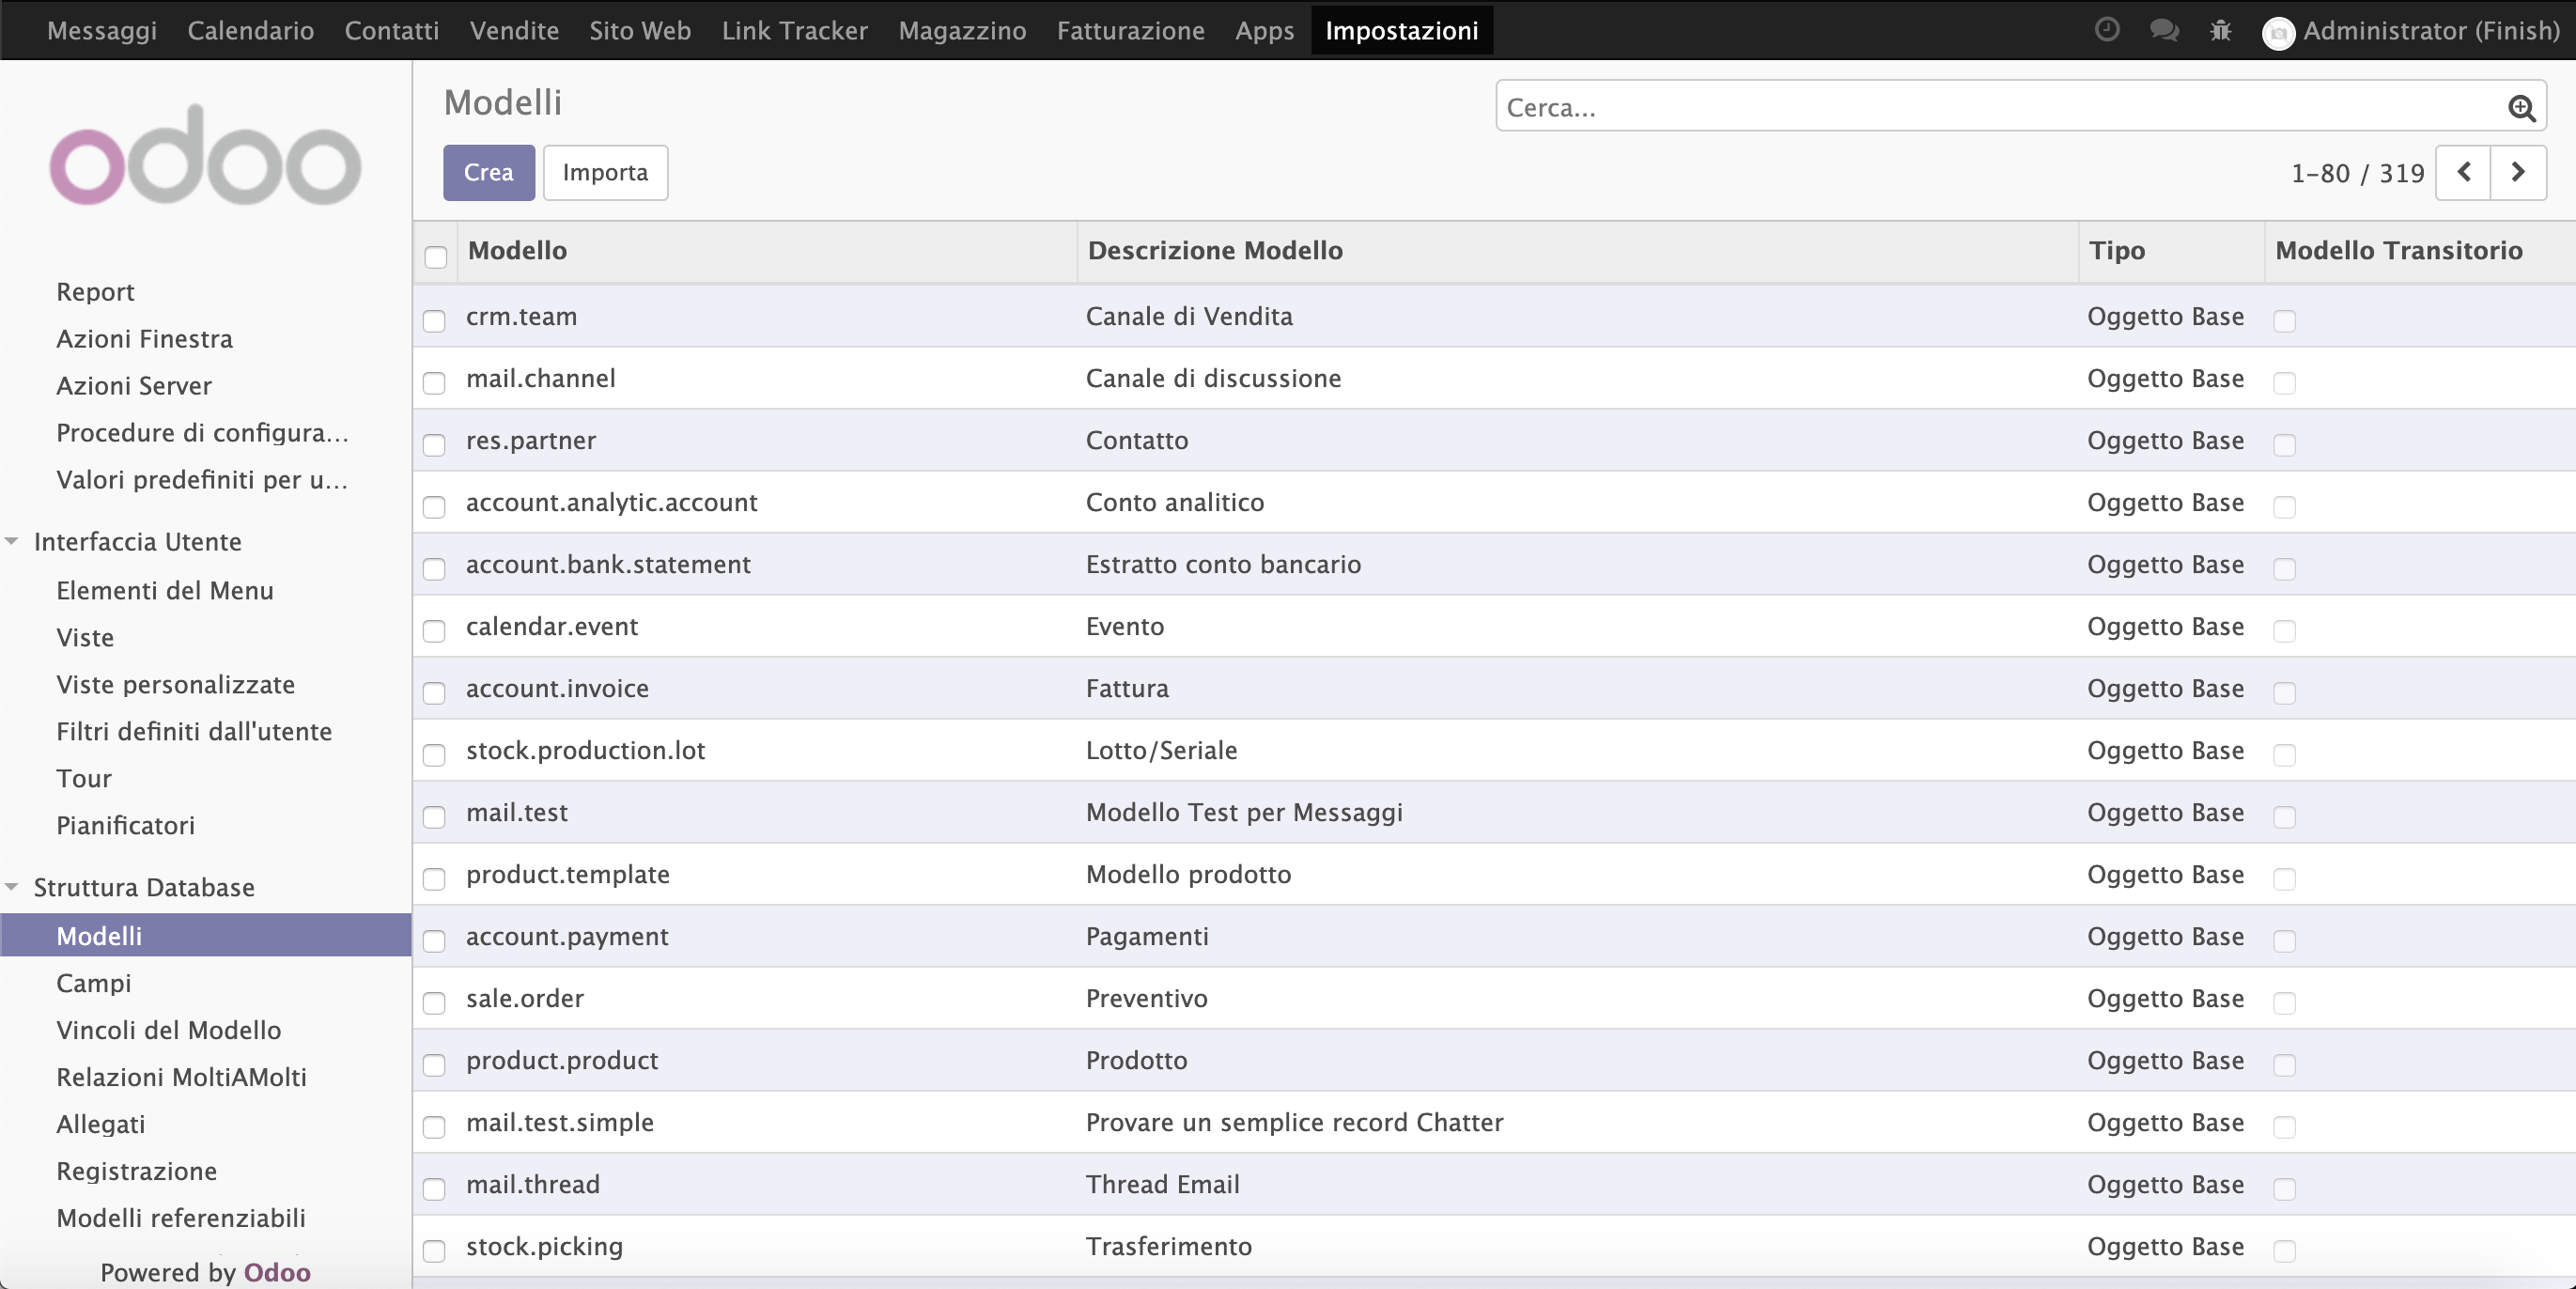
\includegraphics[scale=0.3]{figures/Modelli_creati}
		\caption[Modelli creati]{Modelli creati}
		\label{fig:Modelli_creati}
	\end{center}
\end{figure}
\newpage
\section{Moduli sviluppati}

I moduli estesi e modificati sono: \begin{itemize}
	\item Limite di credito del partner (my\_project);
	\item Canali di Vendita (ibg\_code);
	\item Gestione imballi (ibg\_packaging).
\end{itemize}
\begin{figure}[H]
	\begin{center} 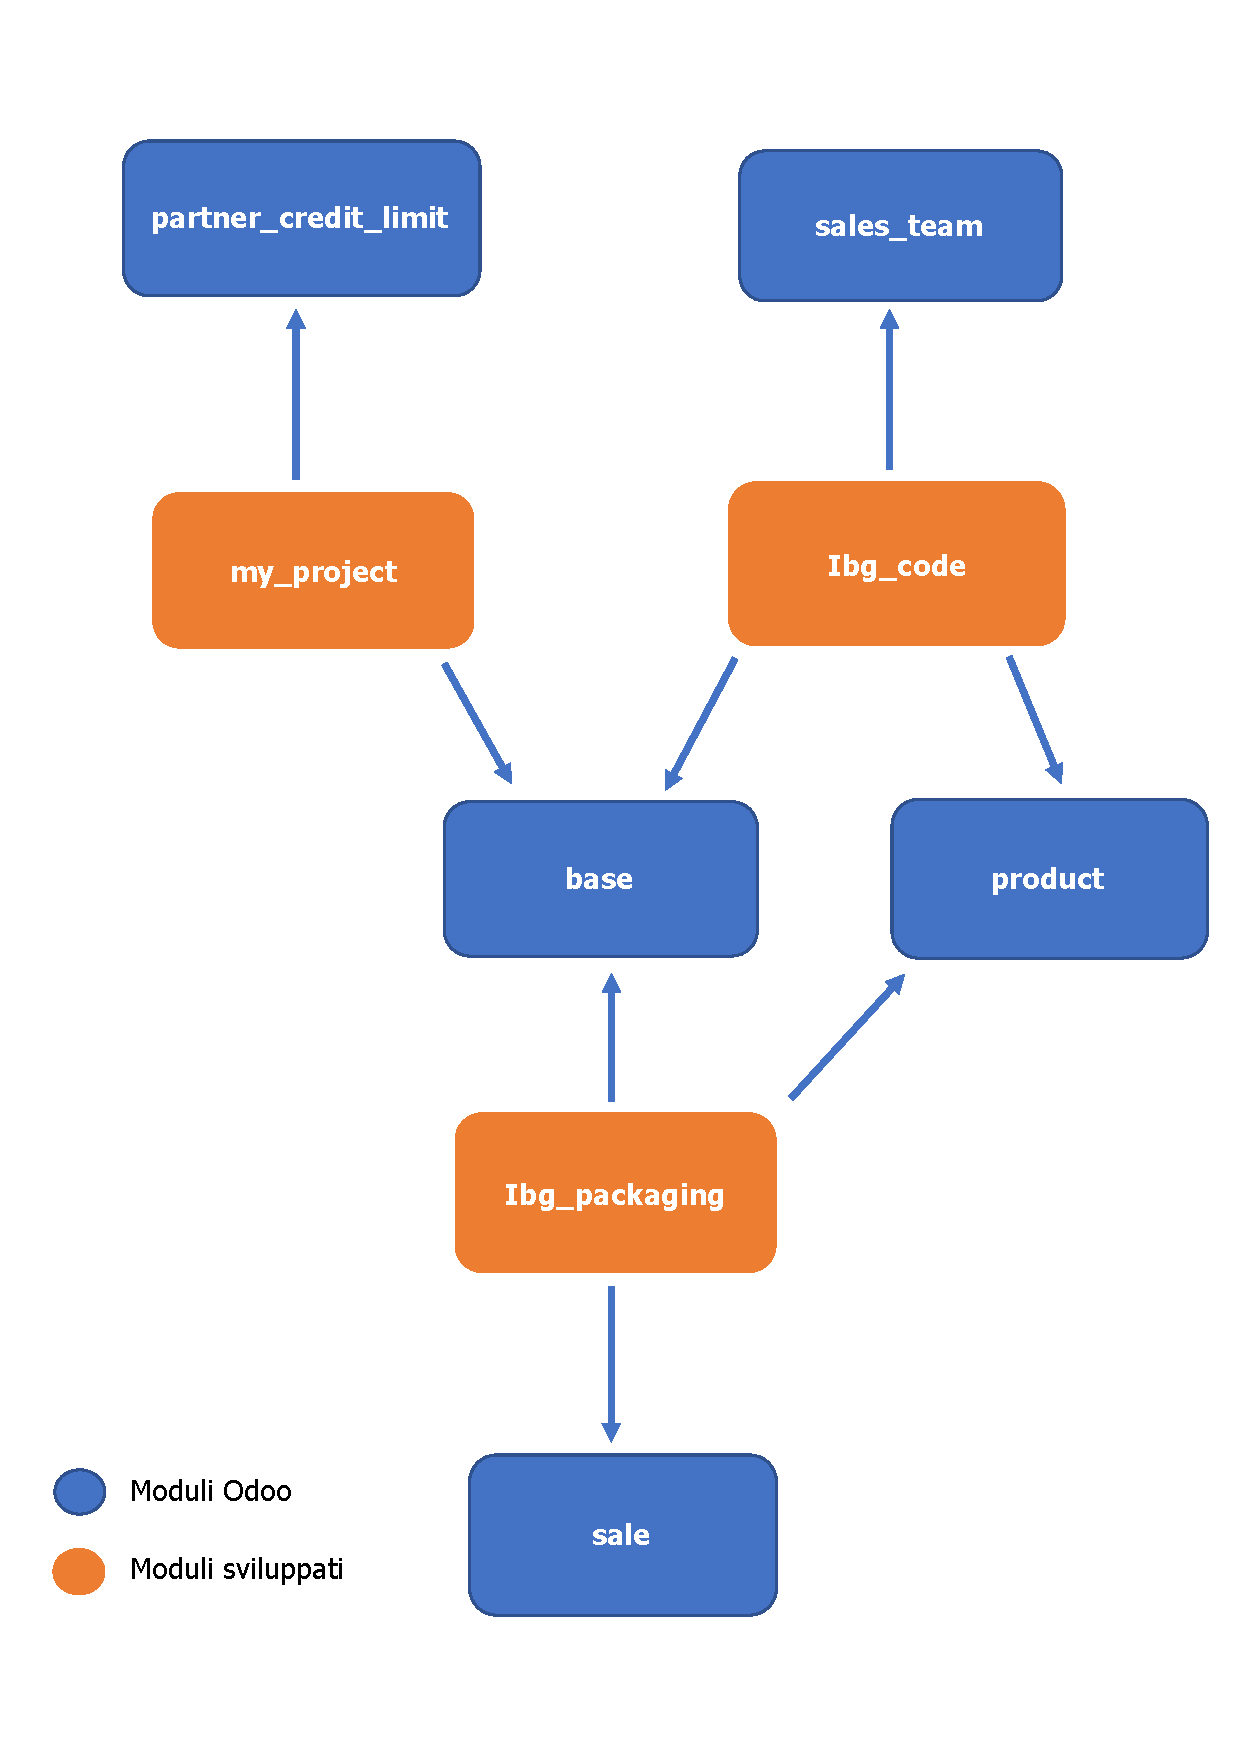
\includegraphics[scale=0.50]{figures/diagramma}
		\caption[Diagramma moduli sviluppati]{Diagramma moduli sviluppati}
		\label{fig:diagramma}
	\end{center}
\end{figure}
\newpage
\subsection{Limite di credito del partner}
Questo modulo entra in funzione quando si approva un ordine di vendita, calcola la somma di:
\begin{itemize}
\item Il credito che il partner deve pagare;
\item L'importo degli ordini di vendita approvati ma non ancora fatturati;
\item L'importo dell'ordine di vendita da approvare e lo confronta con il limite di credito del partner. Se il limite di credito è inferiore, non consente di approvare l'ordine di vendita;
\item Se l'opzione Consenti credito è selezionata, il sistema non controllerà i limiti di credito e consentirà a quel partner di ignorare il limite.
\end{itemize}
\vspace*{0.5cm}
Qui abbiamo aggiunto le seguenti funzionalità.\\
Inseriamo gli stati Blocco Scaduto e Limite di credito.\\
Quando raggiungiamo lo stato Limite di Credito, stiamo confermando un ordine con un importo totale superiore al credito del partner.\\
Al momento della conferma d'ordine verrà mostrato un popup contenente:
\begin{itemize}
	\item Cliente;
	\item Il credito disponibile del partner.
\end{itemize}
\newpage
\begin{figure}[H]
	\begin{center} 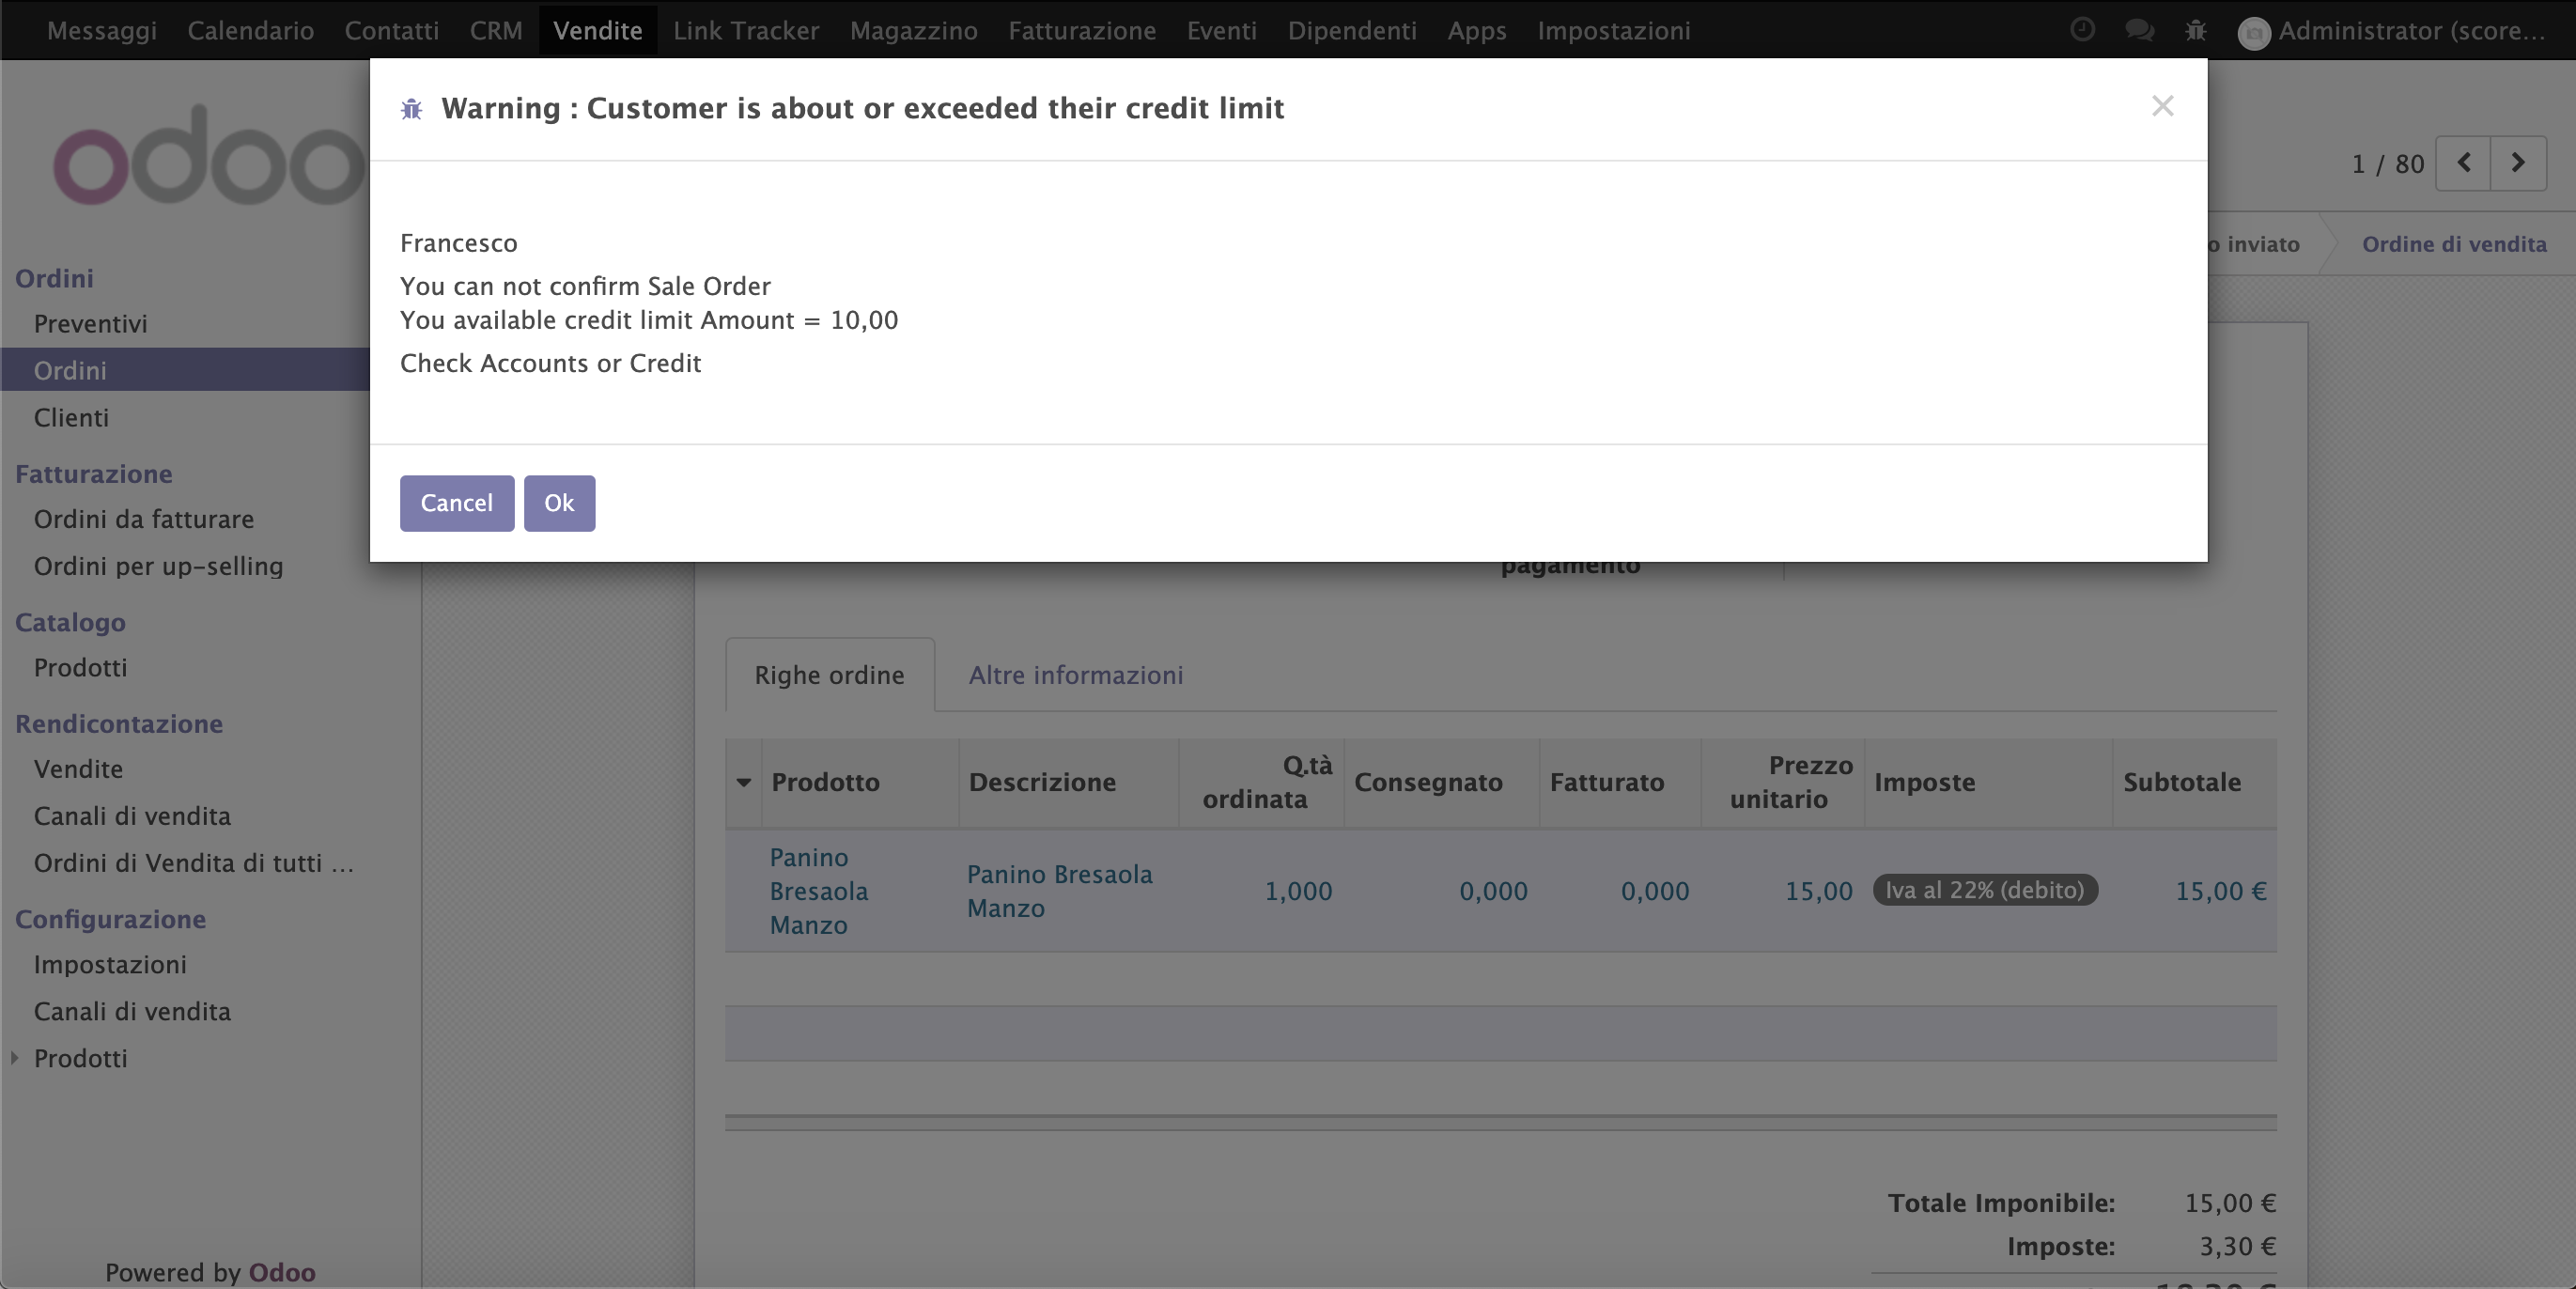
\includegraphics[scale=0.3]{figures/check_limit}
		\caption[Popup limite di credito]{Popup limite di credito}
		\label{fig:check_limit}
	\end{center}
\end{figure}

Al momento del click sul tasto ok, del popup, la fattura si sposterà nello stato Limite di Credito, dove non sarà possibile modificarla, e verrà inviata una mail al direttore commerciale con scritto:\vspace*{0.5cm}\\
\textit{Caro Administrator,\\
	l'ordine di vendita \textbf{n° SO} del cliente \textbf{nome cliente} è stato bloccato per Limite di Credito.\\
	Puoi accedere al SO dal seguente link: \textbf{link al SO di riferimento}.}\vspace*{0.5cm}

Inoltre è stato aggiunto un controllo al momento dell'inserimento di un prodotto. Se cerchiamo di modificare il prezzo unitario (>, < del prezzo di listino) dall'interfaccia 'Righe ordine', salviamo e confermiamo l'ordine, si visualizzerà un popup d'errore con scritto:\\ \textit{Prezzo non idoneo !}
\newpage
Quando raggiungiamo lo stato Blocco Scaduto, stiamo confermando un ordine con una data di scadenza antecedente a quella attuale, vuol dire che l'ordine di vendita è già scaduto.\\
Al momento della conferma d'ordine verrà mostrato un popup contenente:\\
\begin{itemize}
	\item Cliente;
	\item Fatture Scadute: campo contenente l'elenco delle fatture scadute del cliente;
	\item Importo dello scaduto: campo contenente la somma del totale delle fatture scadute;
	\item Button OK
\end{itemize}
\newpage
Inoltre al momento del click del tasto ok del popup, la fattura si sposterà nello stato Blocco Scaduto, dove non sarà possibile modificarla, e verrà inviata una mail al direttore commerciale con scritto:
\vspace*{0.5cm}\\
\textit{Caro Administrator,\\
l'ordine di vendita \textbf{n° SO} del cliente \textbf{nome cliente} è stato bloccato per presenza di pagamenti scaduti.\\
Puoi accedere al SO dal seguente link: \textbf{link al SO di riferimento}.}


\vspace*{1.5cm}
\begin{figure}[H]
	\begin{center} 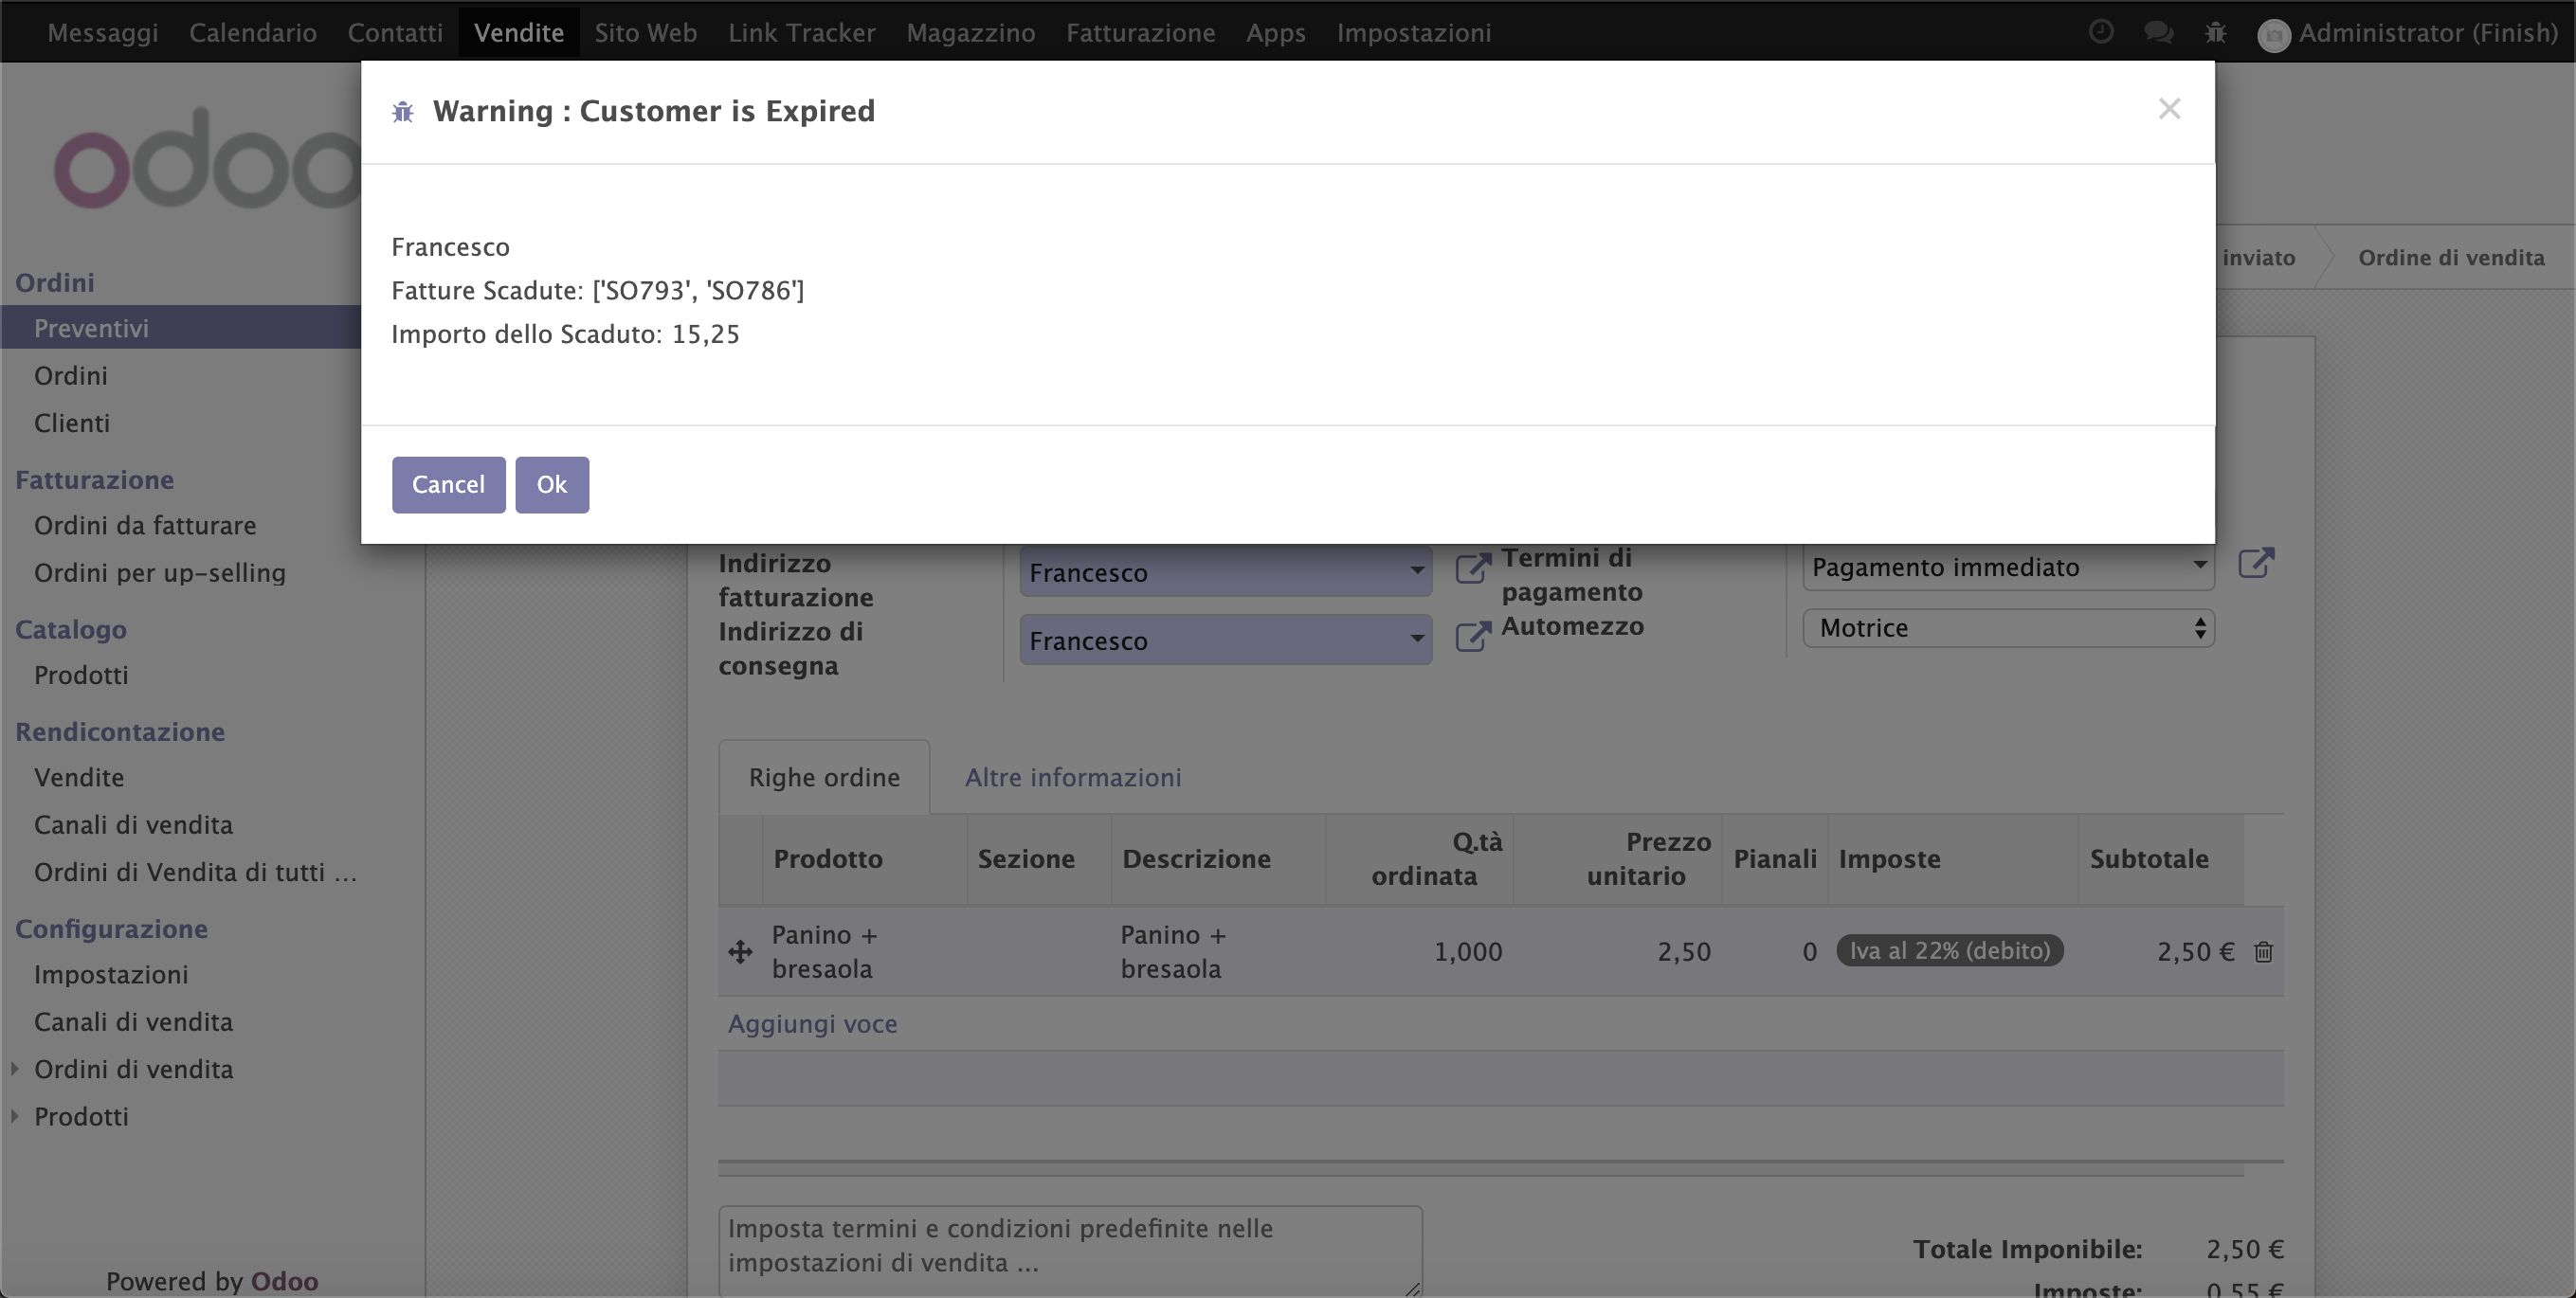
\includegraphics[scale=0.3]{figures/check_expired}
		\caption[Popup blocco scaduto]{Popup blocco scaduto}
		\label{fig:check_expired}
	\end{center}
\end{figure}


\newpage
\section{Canali di Vendita}
Nella sezione Vendite, sulla voce Canali di Vendita abbiamo la possibilità di inserire un nuovo canale.
In questo modulo abbiamo aggiunto al form il campo Codice canale e Codice canale di vendita.
Il campo Codice canale di vendita viene valorizzato con il codice canale + nome del canale di vendita.\\
Poi nella voce Clienti, che fa riferimento ad un altro modulo, quando aggiungiamo un nuovo cliente e selezioniamo 'Persona', abbiamo aggiunto il campo Codice cliente. Questo campo non verrà visualizzato nel momento in cui inserendo un nuovo nuovo cliente selezioniamo azienda.

\begin{figure}[H]
	\begin{center} 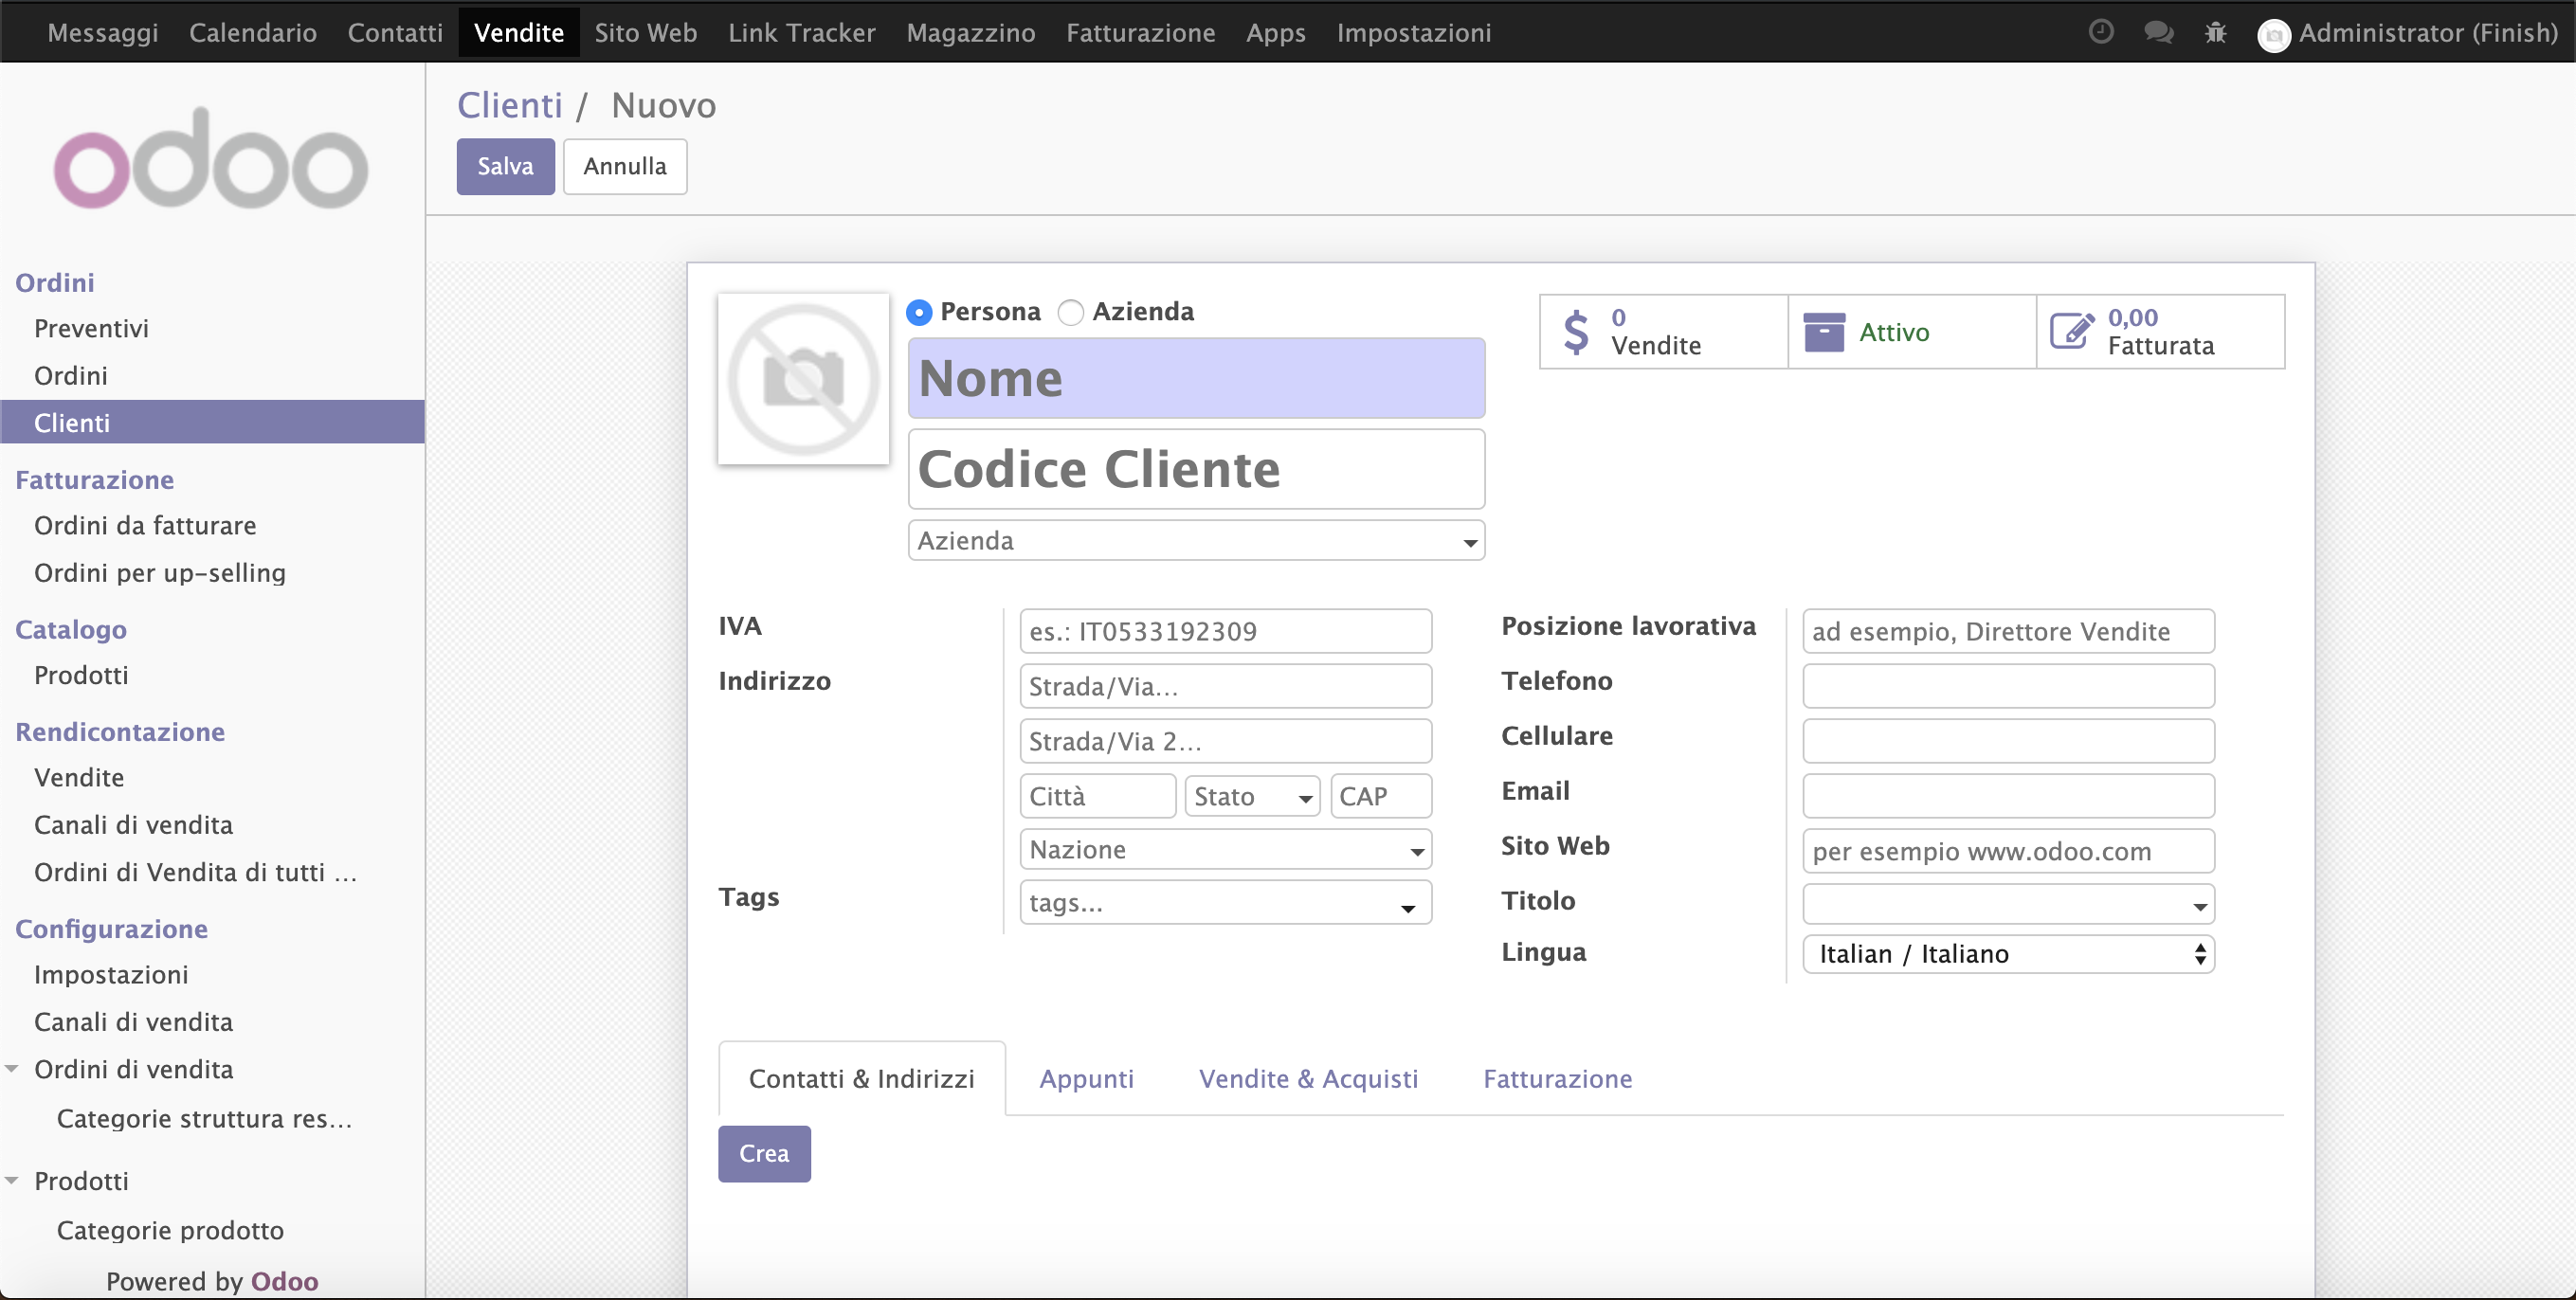
\includegraphics[scale=0.3]{figures/ibg_code}
		\caption[Inserimento nuovo cliente: persona]{Inserimento nuovo cliente: persona}
		\label{fig:ibg_code}
	\end{center}
\end{figure}
\newpage

\section{Gestione imballi}
Nella sezione Magazzino, sulla voce Colli di prodotto abbiamo aggiunto i seguenti campi:
\begin{itemize}
\item Pianale (in relazione con un solo prodotto);
\item Codice Parte (in relazione con un solo prodotto);
\item Bottiglie per cassa;
\item N° pianali per motrice;
\item N° pianali per rimorchio
\end{itemize}

\begin{figure}[H]
	\begin{center} 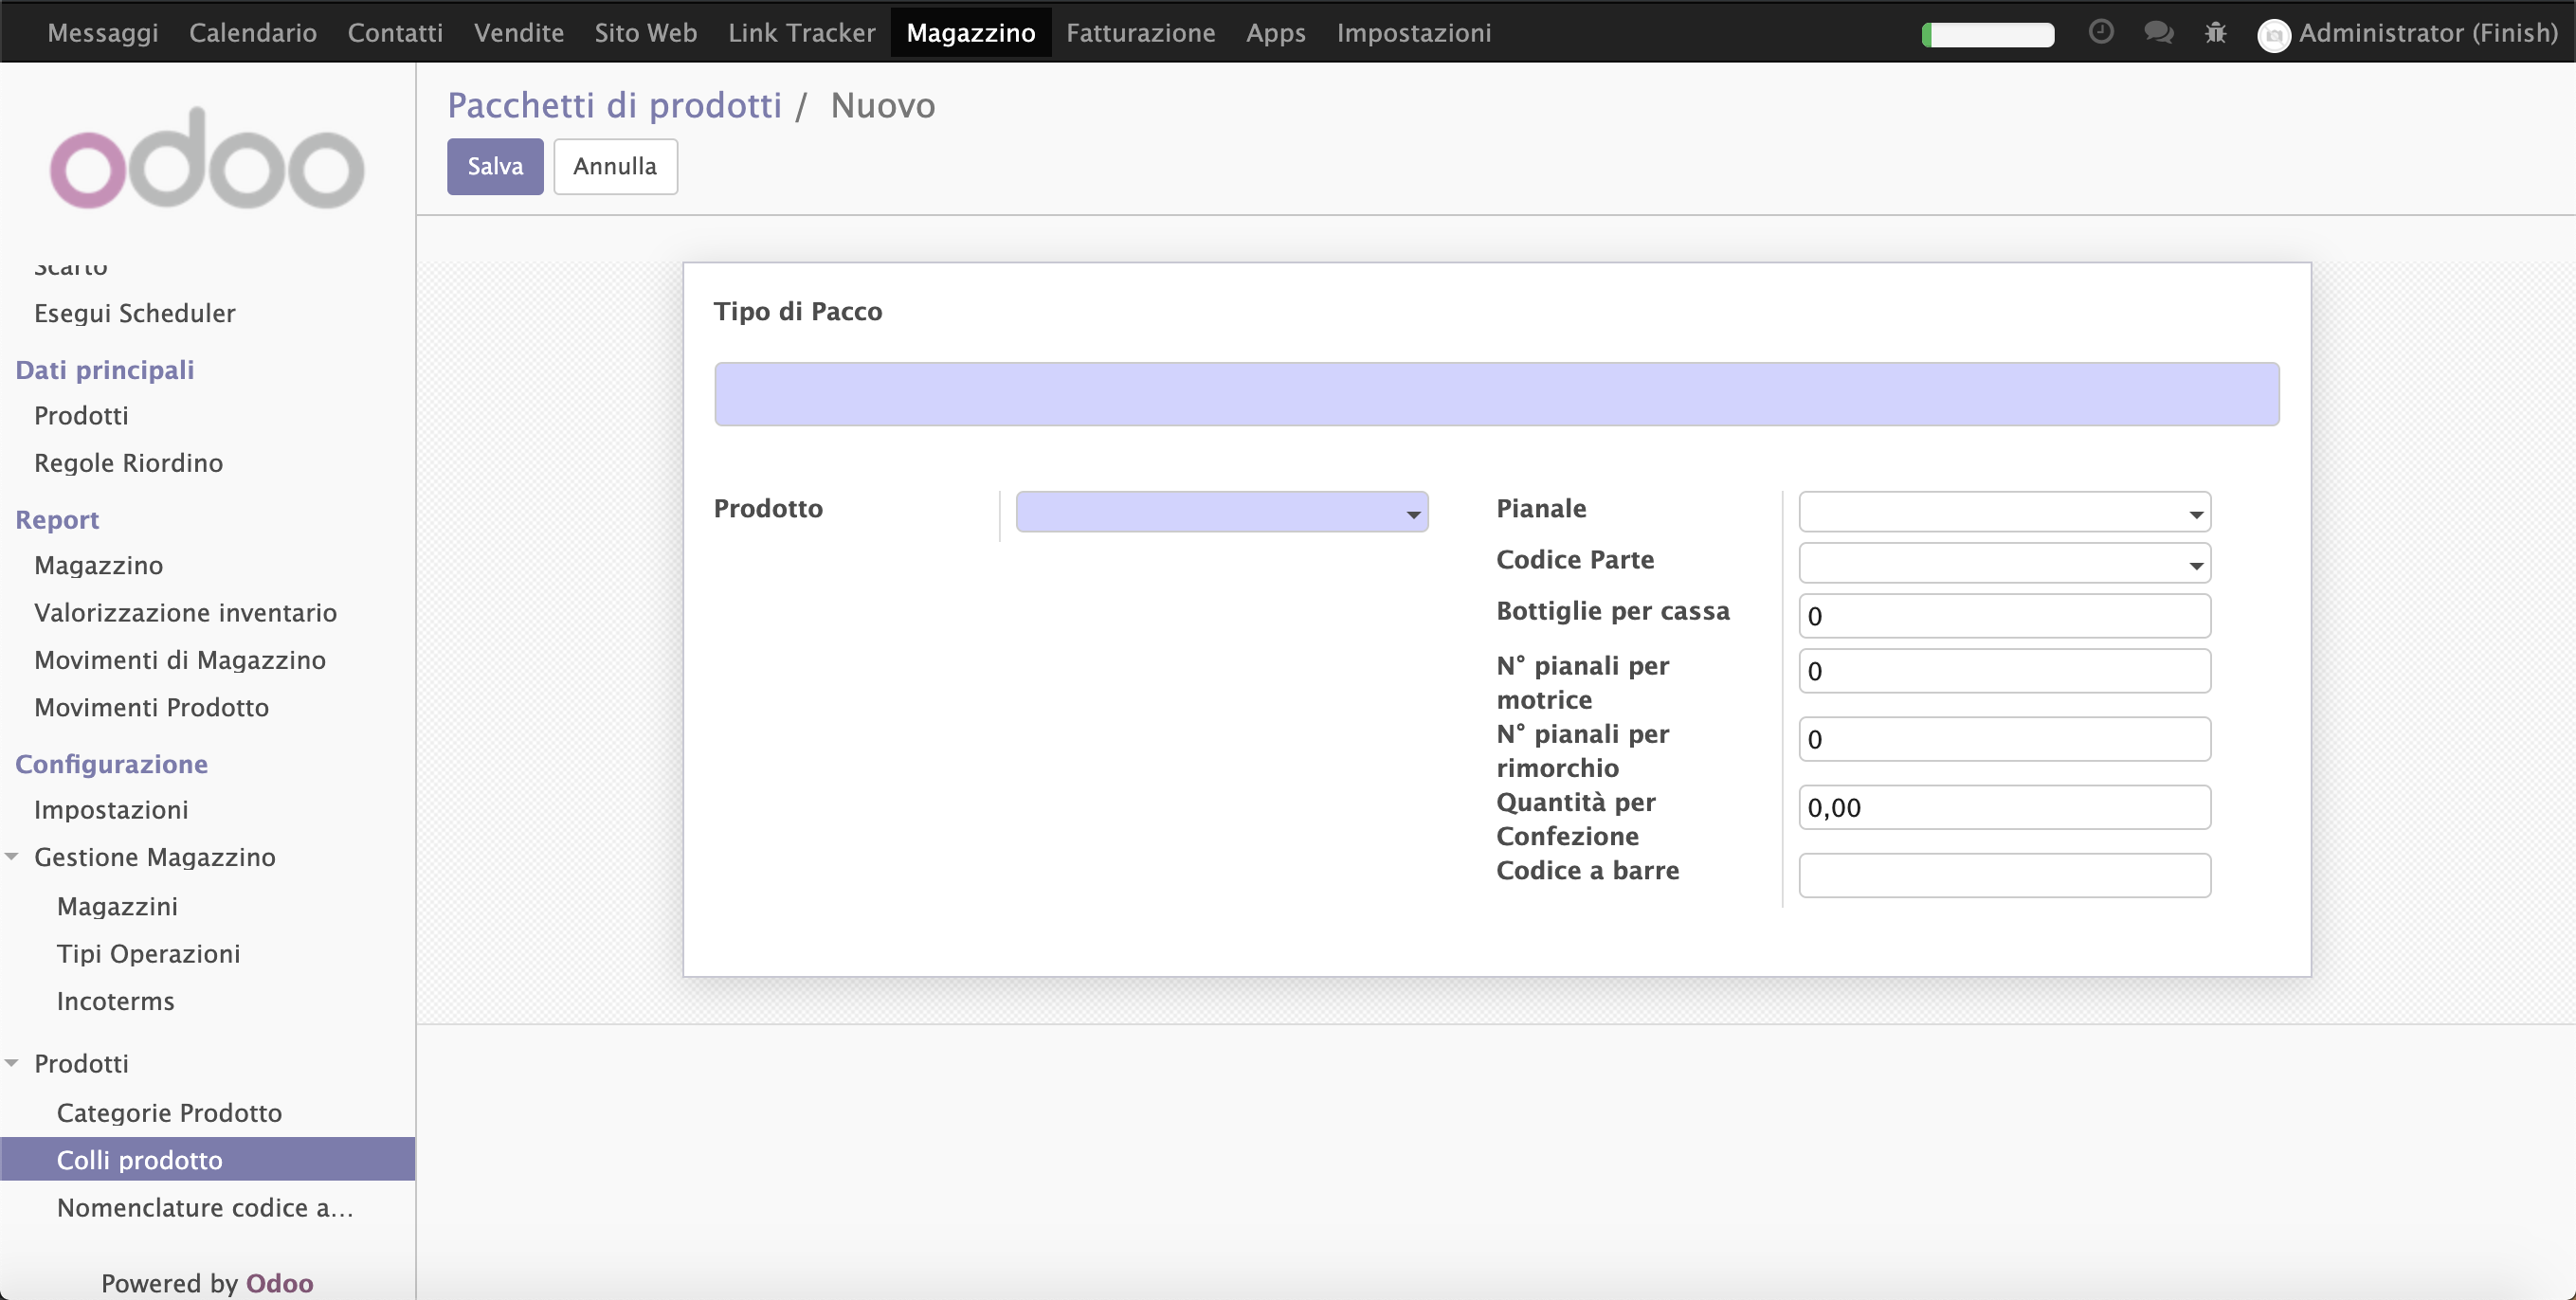
\includegraphics[scale=0.3]{figures/product_packagin}
		\caption[Inserimento pacchetti di prodotti]{Inserimento pacchetti di prodotti}
		\label{fig:product_packagin}
	\end{center}
\end{figure}

Nella sezione Vendite, voce Ordini, abbiamo aggiunto il campo \textit{Pianali}, che viene compilato tramite la divisione tra "quantità ordinata" / "quantità per confezione".
La logica per il calcolo del campo è la seguente:
\begin{itemize}
	\item Se il rapporto da come risultato un numero intero, il sistema deve compilare il campo Pianali con il risultato del rapporto;
	\item Se il rapporto da come risultato un numero decimale inferiore all'unita il campo Pianali va settato a null;
	\\ (Risultato rapproto= 0,5 campo pianali = null)
	\item Se il rapporto da come risultato un numero decimale superiore all'unità il valore del campo Pianali va compilato con il risultato del rapporto approssimato per difetto all'intero più vicino. \\
	(Risultato rapproto= 2,5 campo pianali = 2).
\end{itemize}
Inoltre, abbiamo inserito il seguente campo Automezzo contenente i valori:\\ Autotreno, Motrice. Alla fine di tutto, otteniamo la seguente view.
\vspace*{0.5cm}
\begin{figure}[H]
	\begin{center} 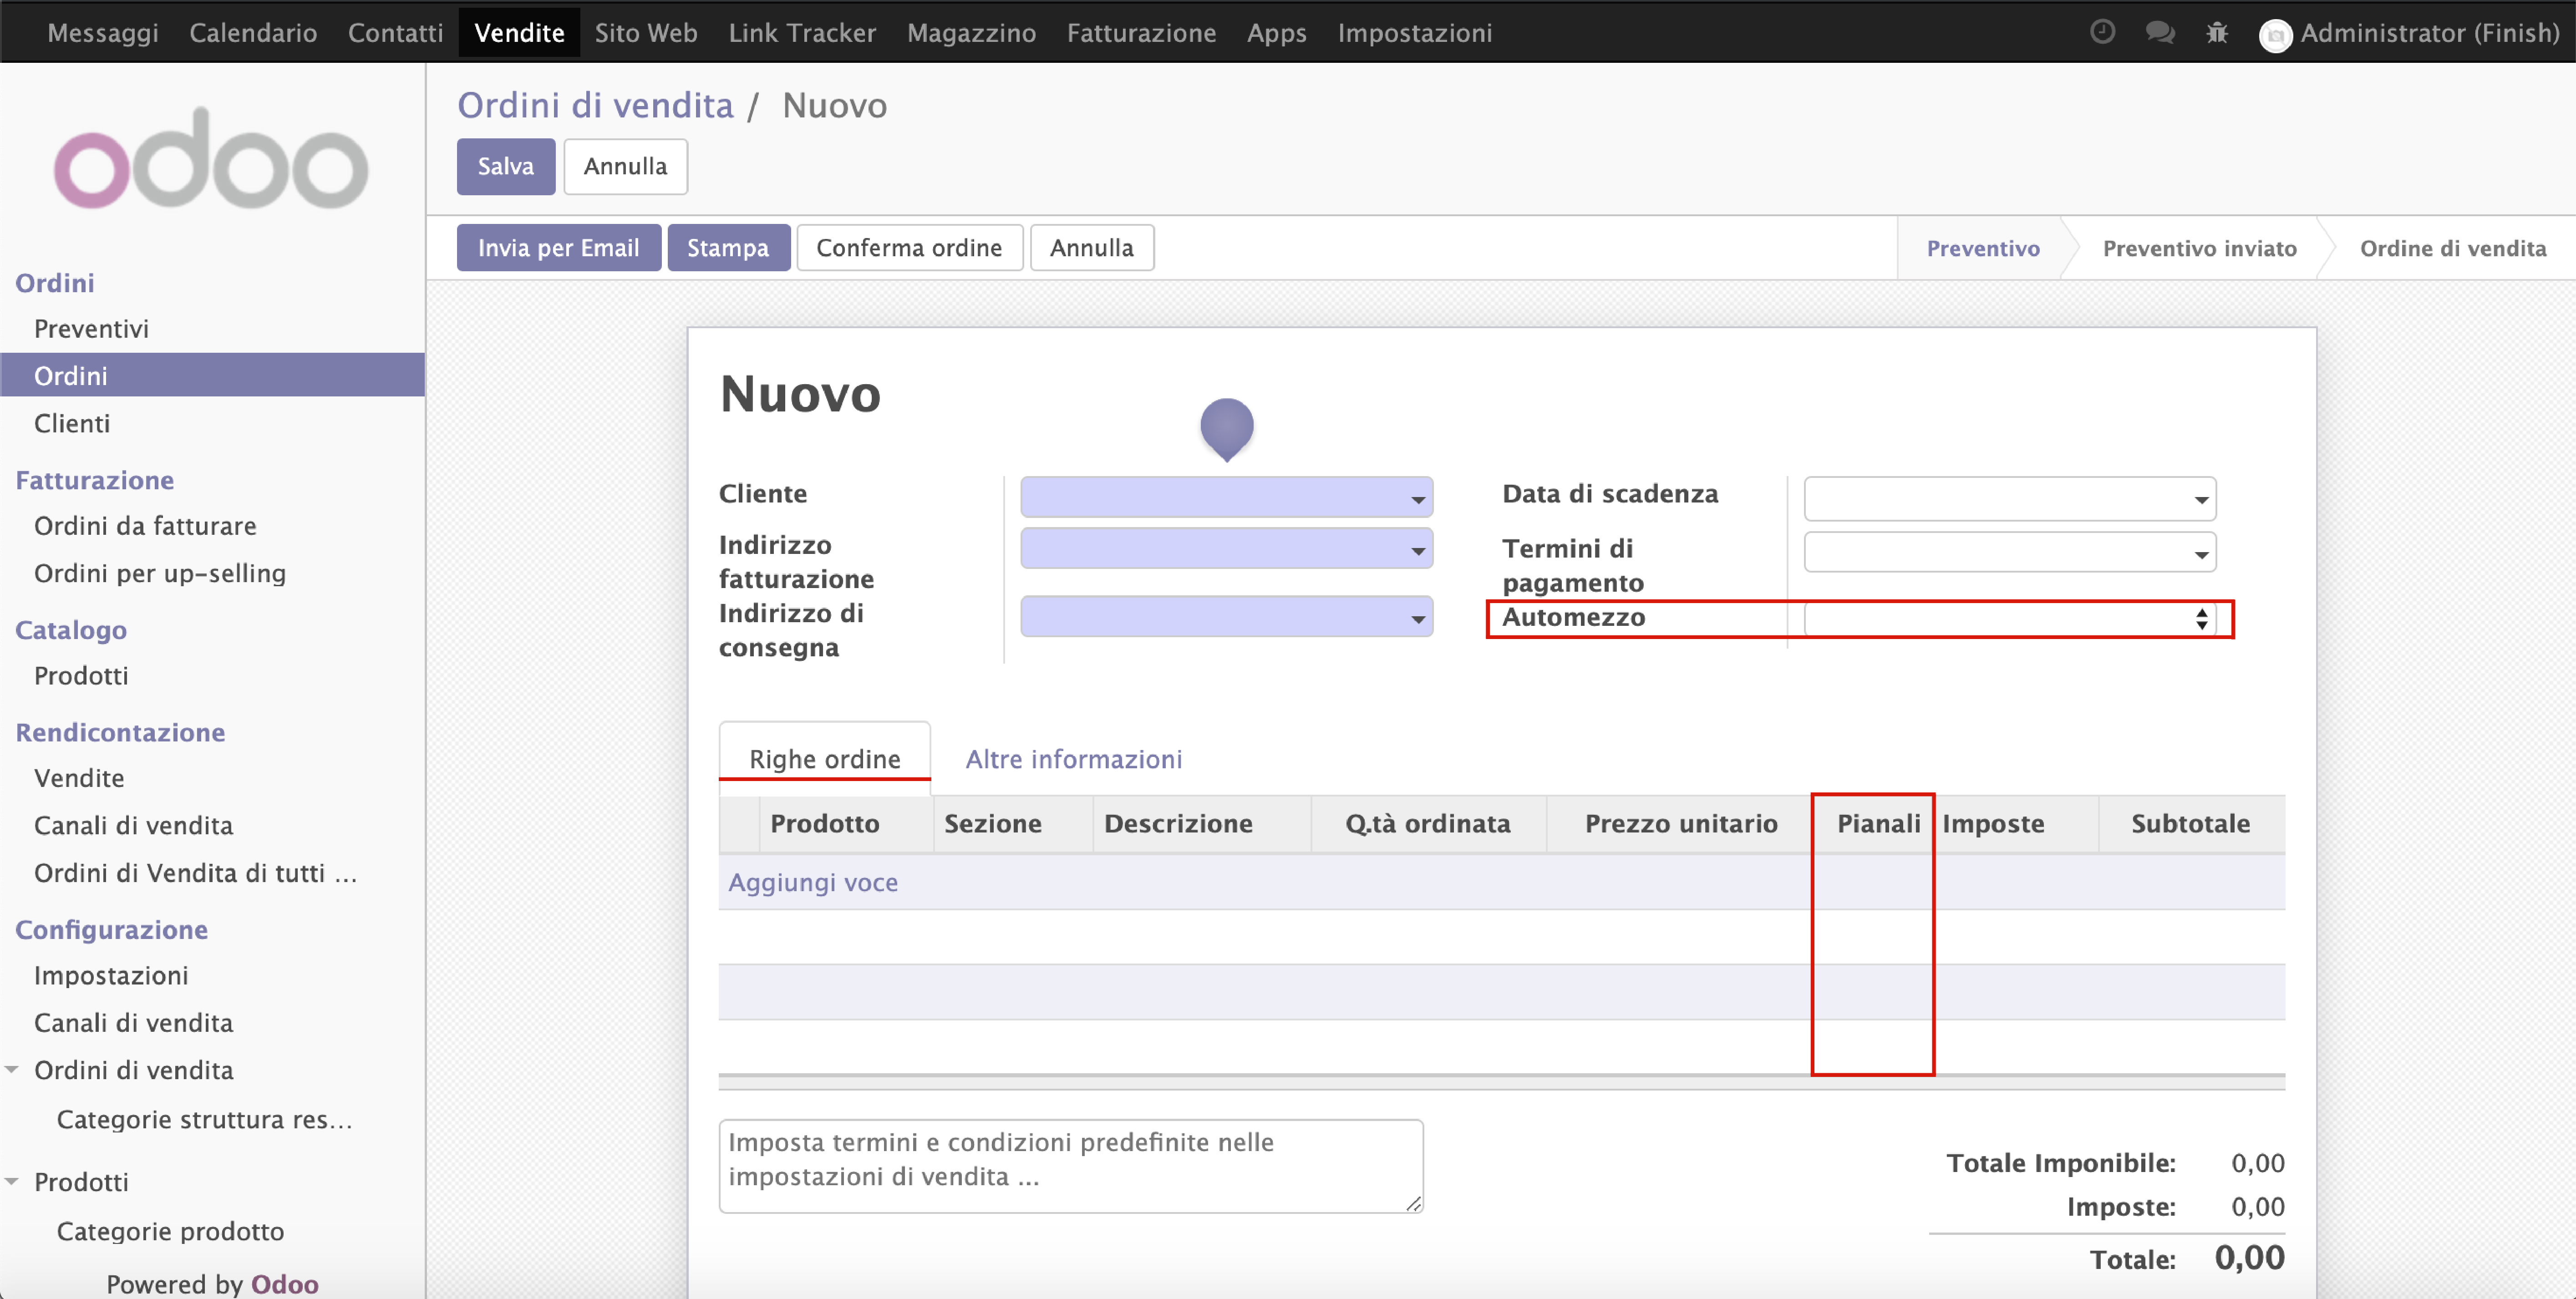
\includegraphics[scale=0.3]{figures/pianali}
		\caption[Campo Pianali e Automezzo in Ordini di vendita]{Campo Pianali e Automezzo in Ordini di vendita}
		\label{fig:pianali}
	\end{center}
\end{figure}

Un'altra funzionalità la troviamo al salvataggio dell'ordine che innesca una funzione che effettua la seguente operazione:
\begin{itemize}
\item Nel caso in cui gli ordini creati nelle righe ordine presentino lo stesso prodotto occorre rendere unica la \textit{line} aggiornando quindi la quantità;
\end{itemize}
\newpage
Infine nel form di inserimento prodotto sono stati aggiunti due campi checkbox: E' un imballo, E' un fustino.

\vspace*{0.5cm}
\begin{figure}[H]
	\begin{center} 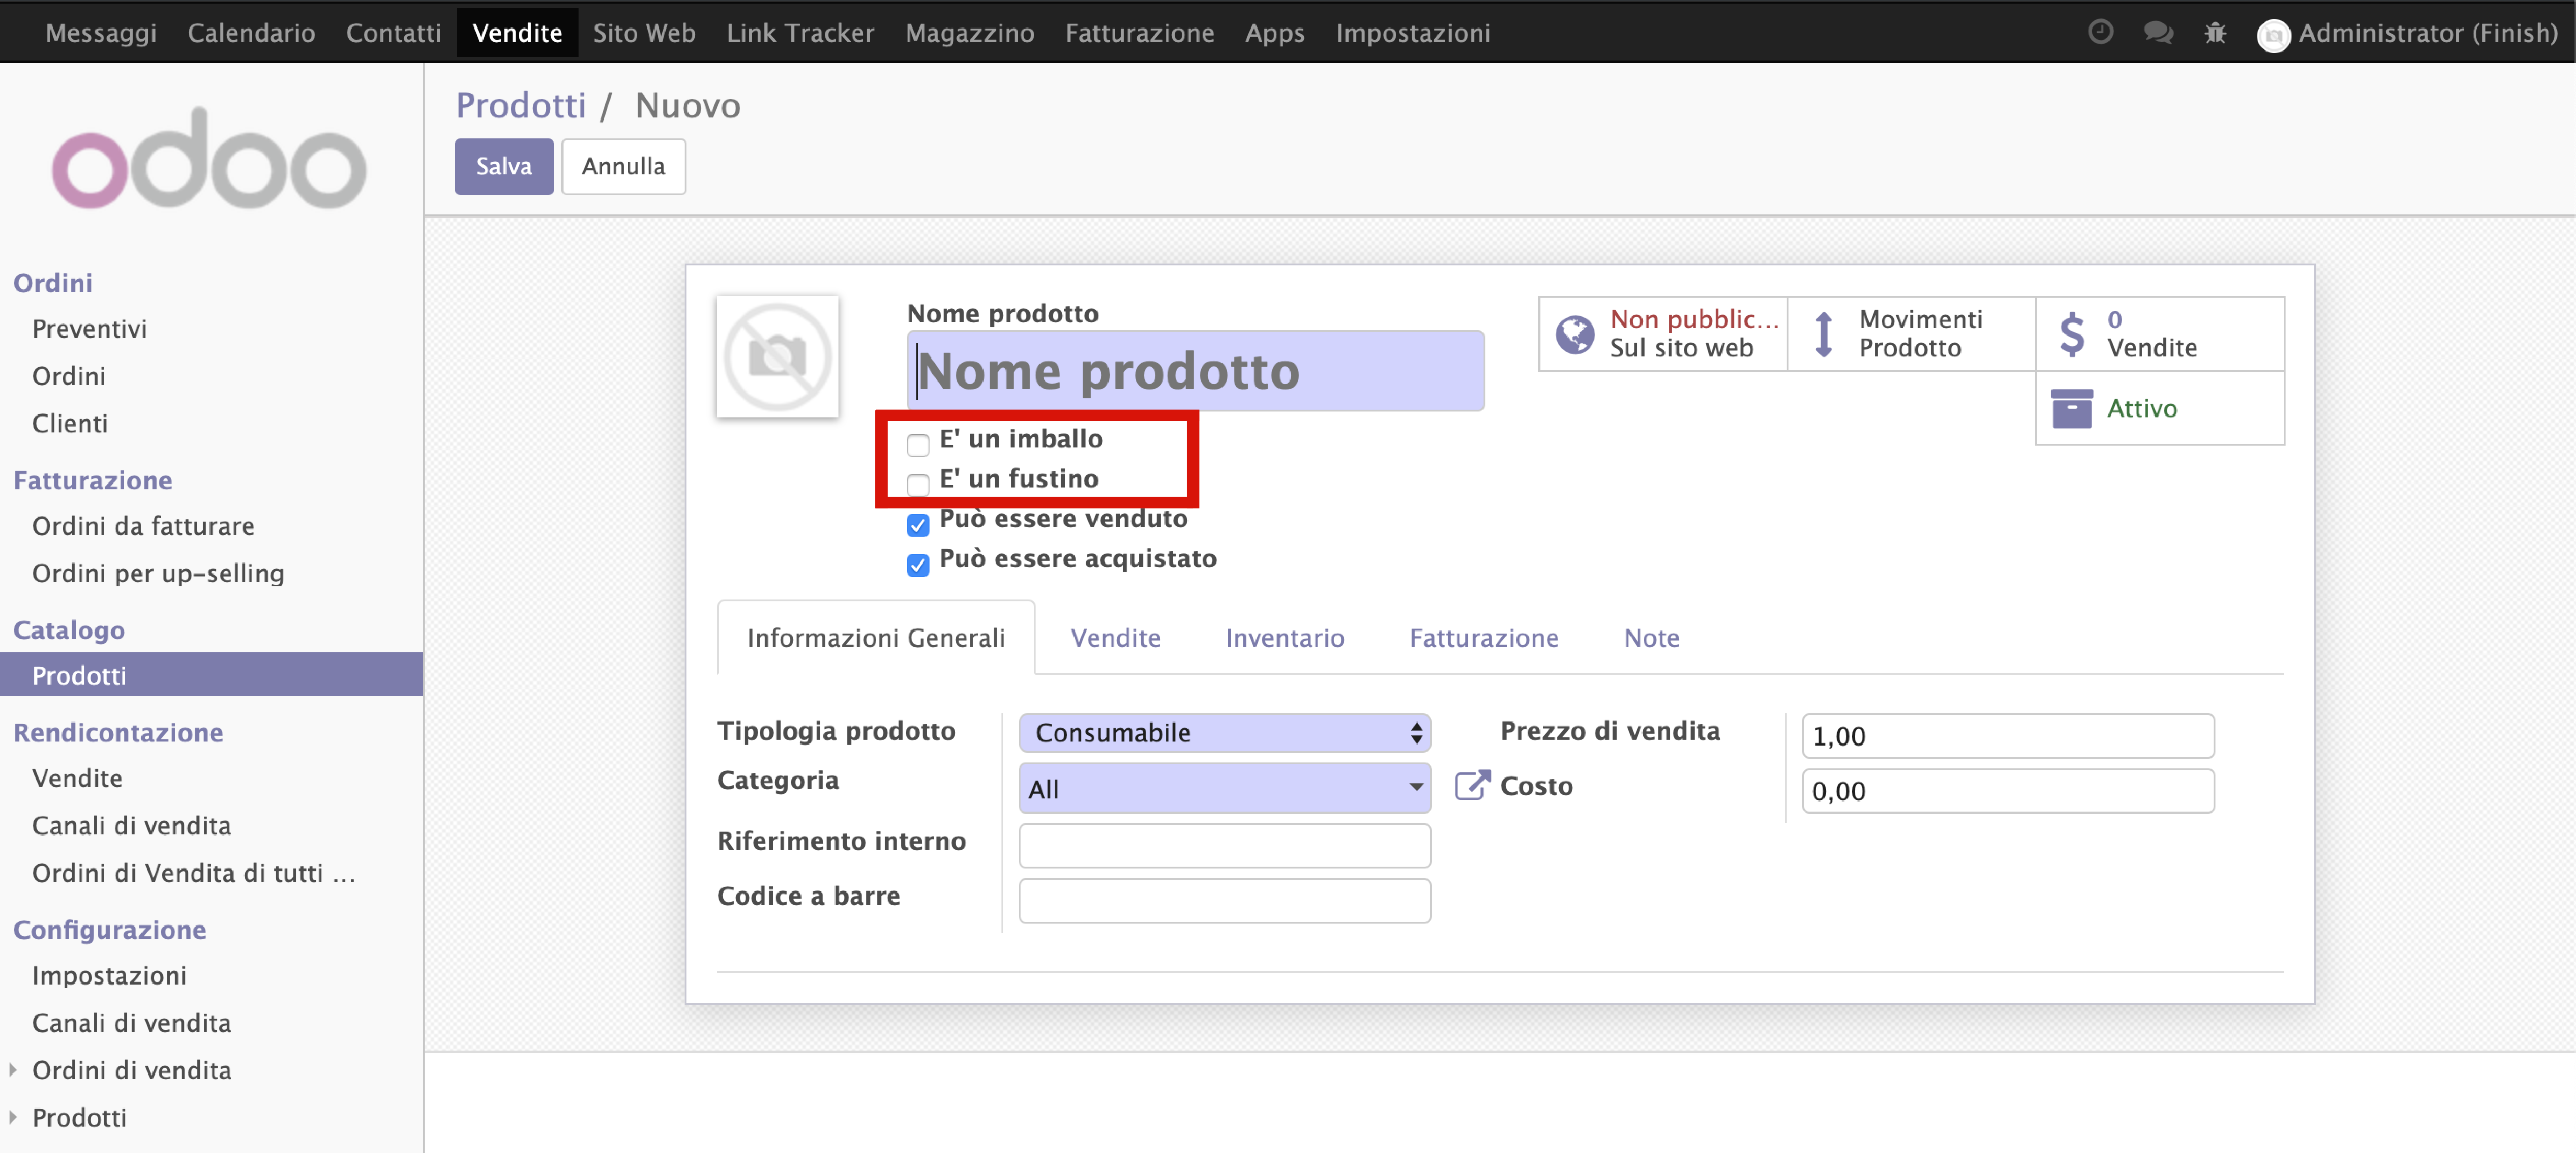
\includegraphics[scale=0.3]{figures/order}
		\caption[Campi checkbox in Prodotti]{Campi checkbox in Prodotti}
		\label{fig:order}
	\end{center}
\end{figure}


